% Report section "Beyond dictatorship" (file 04; label sec:smd).  Input after 02_complementarities.
% Requires \usepackage{wrapfig}.  Proofs and negative results: appendix_smd.tex (app:smd).
% Figure: figures/04_smd.png (generated by experiments/report_figures.py).

\section{Beyond dictatorship: a mechanism that reacts to agreement}
\label{sec:smd}

Theorem~\ref{thm:B} caps every fixed-menu mechanism well below the LP bound, because a dictator
choosing from a fixed menu cannot tell whether the other agent wants the same item (where the
first best pools) or the other one (where it splits). The simplest rule that conditions on
agreement is the following. Let $\tau=(1+\varepsilon)/2$ and $s\in[0,1]$.

\begin{definition}[SMD: split if strongly opposed, else modest dictator]
If $x\ge\tau$ and $y\le1-\tau$, or $y\ge\tau$ and $x\le1-\tau$, each agent receives her preferred
item in full. Otherwise a fair coin picks a dictator, who receives a share $s$ of her preferred
item; the other agent receives the rest.
\end{definition}

\begin{proposition}[strategy-proofness]\label{prop:D}
SMD is strategy-proof for every $s\in[0,1]$ and $\varepsilon\in[0,1]$.
\end{proposition}
\noindent The report matters only against a strongly opposed opponent; there, the split is worth
$x$ to an agent preferring item~1 and the coin flip is worth $xs+\tfrac12(1-s)(1+\varepsilon)$, and the
two cross exactly at $x=\tau$, so strong types prefer the split and moderate types the coin flip,
which is what truthful reporting gives each of them (Appendix~\ref{app:smd}).

\begin{wrapfigure}{r}{0.45\linewidth}
\centering
\vspace{-1ex}
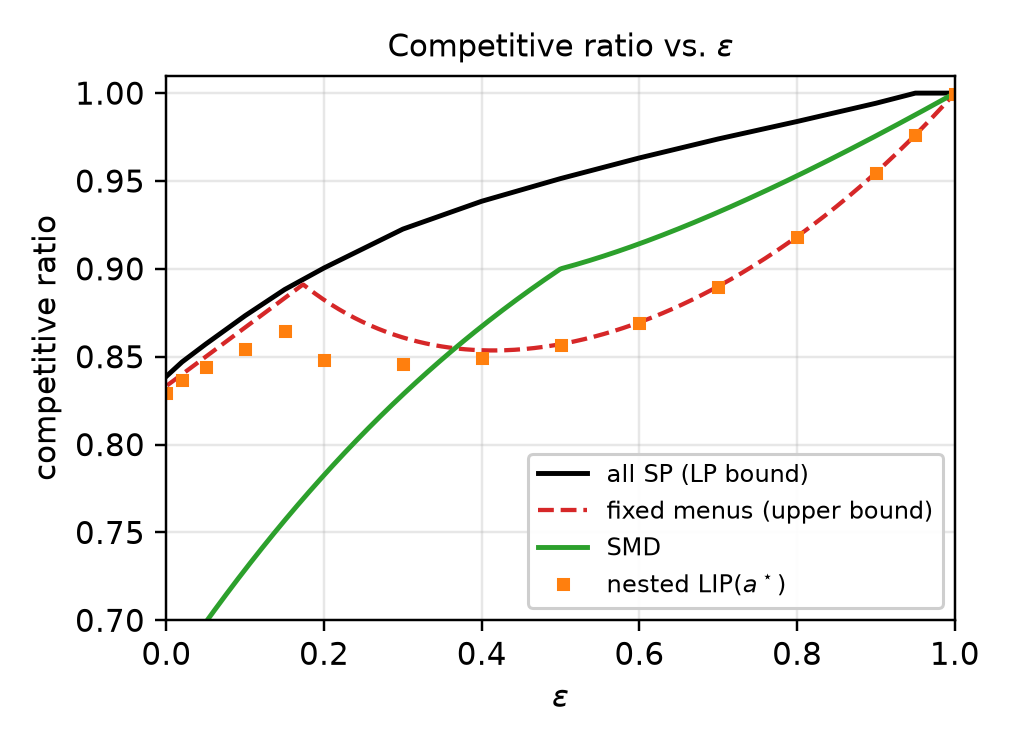
\includegraphics[width=\linewidth]{figures/04_smd.png}
\caption{SMD with the optimal share $s^\star$ against the closed-form bound on fixed-menu mechanisms
(Theorem~\ref{thm:B}, dashed), nested LIP with optimised $a$, and the LP bound on all
strategy-proof mechanisms ($N\le80$).}
\label{fig:smd}
\vspace{-2ex}
\end{wrapfigure}

\begin{proposition}[competitive ratio]\label{prop:E}
With the optimal share $s^\star$, SMD is exactly $\rho_{\mathrm{SMD}}$-competitive, where
\[
\rho_{\mathrm{SMD}}(\varepsilon)=\frac{2(1+\varepsilon)^2}{3+3\varepsilon+2\varepsilon^2}\ \ (\varepsilon\le\tfrac12),
\qquad
\rho_{\mathrm{SMD}}(\varepsilon)=\frac{(1+\varepsilon)^2}{1+3\varepsilon}\ \ (\varepsilon\ge\tfrac12).
\]
\end{proposition}
\noindent Two profiles bind: identical preferences, where the first best pools and a larger $s$
hurts, and the edge of the split region ($x=1$, $y=(1-\varepsilon)/2$), where the coin flip
should give more and a larger $s$ helps; $s^\star$ equalises them ($s^\star=0.3$ at $\varepsilon=\tfrac12$).

SMD gives $0.867$, $0.900$ and $0.942$ at $\varepsilon=0.4$, $0.5$ and $0.75$, against $6/7\approx0.857$
and $28/31\approx0.903$ for the best fixed menu at $\varepsilon=0.5$ and $0.75$. It exceeds every
fixed-menu mechanism for $\varepsilon>0.366$ (Figure~\ref{fig:smd}), so with complementarities a
mechanism that uses both reports jointly beats the paper's entire class. Below $\varepsilon\approx0.37$
the menus (and nested LIP) remain the best mechanisms we have.

The rule is rigid: a larger threshold, a probabilistic split for moderately opposed agents,
or nested LIP as the fallback all break strategy-proofness, and optimising the fallback menu by
an LP helps only for $\varepsilon\lesssim0.45$ (Appendix~\ref{app:smd}). A gap of about $0.05$ to the
LP bound remains at $\varepsilon=\tfrac12$ ($0.900$ vs $0.951$). The LP-optimal mechanisms pool with a
probability that varies smoothly with both types; turning that into a mechanism that is
strategy-proof on the whole continuum is the main open question this project leaves.
